\documentclass[9pt]{beamer}

\usetheme[progressbar=frametitle]{metropolis}
\usepackage{appendixnumberbeamer}
\usepackage[style=authoryear, backend=bibtex8, natbib=true, maxcitenames=2]{biblatex}

\usepackage{graphicx}
\usepackage{import}

\usepackage{booktabs}
\usepackage[scale=2]{ccicons}

\usepackage[utf8]{inputenc}

\usepackage{pgfplots}
\usepgfplotslibrary{dateplot}

\usepackage{xspace}
\newcommand{\themename}{\textbf{\textsc{metropolis}}\xspace}

\usepackage{amsmath}
\usepackage{ulem} % use the "sout" tag to "strikethrough" text

\usepackage[super,negative]{nth} % allows writing 1st, 2nd, 3rd with superscript

  % Put % before of what you want disabled

  % Select what to do with todonotes: i.e. \todo{}, \todo[inline]{}
  % \usepackage[disable]{todonotes} % notes not showed
  \usepackage[draft]{todonotes}   % notes showed

  % Select what to do with command \comment:
   \newcommand{\comment}[1]{}  %comment not showed
  % \newcommand{\comment}[1]{\par {\bfseries \color{blue} #1 \par}} %comment showed

  % \makeatletter
  % \renewcommand*{\@textcolor}[3]{%
  %   \protect\leavevmode
  %   \begingroup
  %     \color#1{#2}#3%
  %   \endgroup
  % }
  % \makeatother


\addbibresource{bib_rdd}

\numberwithin{equation}{section}

\title{Application of Regression Discontinuity Design}
\subtitle{The impact of tracking in Kenyan primary schools}
% \date{\today}
\date{\today}
\author{Thor Donsby Noe}
\institute{Analysis \& Evaluation of Public Policies}
%\institute{Department of Economics, University of Copenhagen}
% \titlegraphic{\hfill
\includegraphics[height=1.5cm]{logo.pdf}}

    % \definecolor{BlueTOL}{HTML}{222255}
    \definecolor{BrownTOL}{HTML}{666633}
    \definecolor{GreenTOL}{HTML}{225522}
    % \setbeamercolor{normal text}{fg=BlueTOL,bg=white}
    \setbeamercolor{alerted text}{fg=BrownTOL}
    \setbeamercolor{example text}{fg=GreenTOL}

    \setbeamercolor{block title alerted}{use=alerted text,
        fg=alerted text.fg,
        bg=}
    \setbeamercolor{block body alerted}{use={block title alerted, alerted text},
        fg=alerted text.fg,
        bg=}
    \setbeamercolor{block title example}{use=example text,
        fg=example text.fg,
        bg=}
    \setbeamercolor{block body example}{use={block title example, example text},
        fg=example text.fg,
        bg=}

    \setbeamercolor{block title alerted}{use=alerted text,
        fg=alerted text.fg,
        bg=alerted text.bg!80!alerted text.fg}
    \setbeamercolor{block body alerted}{use={block title alerted, alerted text},
        fg=alerted text.fg,
        bg=block title alerted.bg!50!alerted text.bg}
    \setbeamercolor{block title example}{use=example text,
        fg=example text.fg,
        bg=example text.bg!80!example text.fg}
    \setbeamercolor{block body example}{use={block title example, example text},
        fg=example text.fg,
        bg=block title example.bg!50!example text.bg}


\begin{document}
\setbeamercolor{background canvas}{bg=white}
\maketitle


% ------------------------------------------------------------------------------
% ------ FRAME -----------------------------------------------------------------
% ------------------------------------------------------------------------------
\begin{frame}{Outline}
  \tableofcontents

\end{frame}


\section{Motivation}

\begin{frame}{Introduction}
  Duflo, E., P. Dupas, \& M. Kremer (2011) "Peer Effects, Teacher Incentives, and the Impact of Tracking: Evidence from a Randomized Evaluation in Kenya". In \textit{American Economic Review}, 101: 1739-1774.

  \textbf{Def. 'Tracking':} splitting up pupils according to prior achievements

  Evidence from \textbf{studies in the U.S.}
  \begin{itemize}
    \item High-achieving pupils are widely regarded to gain from tracking
    \item Low-achieving pupils should be affected ambiguously
    \begin{itemize}
      \item[$\downarrow$] Less direct student-to-student spillovers (Epple, Newlon \& Romano \citeyear{epple2002ability}).
      \comment{Which Epple, Newlon and Romano find to dominate in the US.}
      \item[$\uparrow$] Indirect effect: Teacher chooses an instruction level closer to pupil's ability \citep{figlio2002school, zimmer2003new, lefgren2004educational}.
      \comment{Figlio and Lefgren find the two effects to cancel out, Zimmer finds the indirect effect to dominate.}
    \end{itemize}
    \item Mid-achieving pupils are divided by the median $\rightarrow$ \textbf{discontinuity}\\
    Just below the median:
    \begin{itemize}
      \item[$\downarrow$] Less direct student-to-student spillovers.
      \item[$\downarrow$] If teachers always target the middle of a class: Negative indirect effect.
    \end{itemize}
  \end{itemize}
Surprising result of \textbf{randomized experiment} in Kenyan primary schools:
\begin{itemize}
  \item[$\rightarrow$] \citet{duflo2011peer} find that \textit{all} quartiles receive a net benefit from tracking compared to the control group.
\end{itemize}
\end{frame}

\section{Background}

\begin{frame}{Primary education in Kenya}
  Characteristics
  \begin{itemize}
    \item Centralized education system
    \begin{itemize}
      \item National exams.
      \item Curriculum benefitting only high-achieving pupils \citep{glewwe2009many}.
    \end{itemize}
    \item Most teachers are hired centrally through the civil service
    \begin{itemize}
      \item Face weak incentives \citep{duflo2011peer}.
    \end{itemize}
    \item A minority of teachers are hired locally on short-term contracts.
    \begin{itemize}
      \item Face strong incentives $\rightarrow$ good track record can lead to a civil-service job.
    \end{itemize}
    \item Kenya recently abolished school fees $\rightarrow$ huge heterogeneity in pupils.
    \begin{itemize}
      \item Many \nth{1} generation learners.
      \item Few have attended preeschools (costly and optional).
    \end{itemize}
  \end{itemize}
  Incentives to target teaching to the top of the class
  \begin{itemize}
    \item Scores of own pupils in exit exam: A high rate drop out or repeat grades.
    \item Teachers are more likely to interact with parents of top-achievers.
    \comment{As they're more similar}
  \end{itemize}
\end{frame}


\begin{frame}{Experimental design}
  In 2005 grants secured an extra teacher for 18 months in 121 primary schools in Western Kenya with a single \nth{1} grade class that was split into two classes.
  \comment{140 schools, but 19 are excluded from analysis due to having more than 1 first-grade class $\rightarrow$ Sampling bias: Only smaller schools (one \nth{1} grade).}

  \textbf{Random assignment into treatment:}
    \begin{itemize}
      \item[T=1:] \textbf{Tracking schools:} Students were assigned to each of the two classes based on prior test scores, i.e. above median or below median (60 schools).
      \item[T=0:] \textbf{Non-tracking schools:} Students were randomly assigned to either of the two classes (61 schools).
      \item[-] Contract teachers and civil-service teachers were randomly assigned.
    \end{itemize}
  \textbf{Non-compliers and attrititon}
    \begin{itemize}
      \item Many teachers did not comply to assignment
      \begin{itemize}
        \item[$\rightarrow$] 10-14\% of schools had to combine the classes again.
      \end{itemize}
      \item Only a handful of pupils were reassigned due to parent's request.
      \begin{itemize}
        \item 92-96\% of pupils were found in their assigned class (on 5 unannounced visits to each school).
        \comment{Regardless, the analysis is based on the initial assignment.}
        \item 21-23\% of students repeated \nth{1} grade. 0.5\% dropped out.
        \item Attrition rates: 18\% for endline test, 22\% one year after ended treatment.
      \end{itemize}
    \end{itemize}
\end{frame}

\begin{frame}{Very different prior achievement of class mates}
  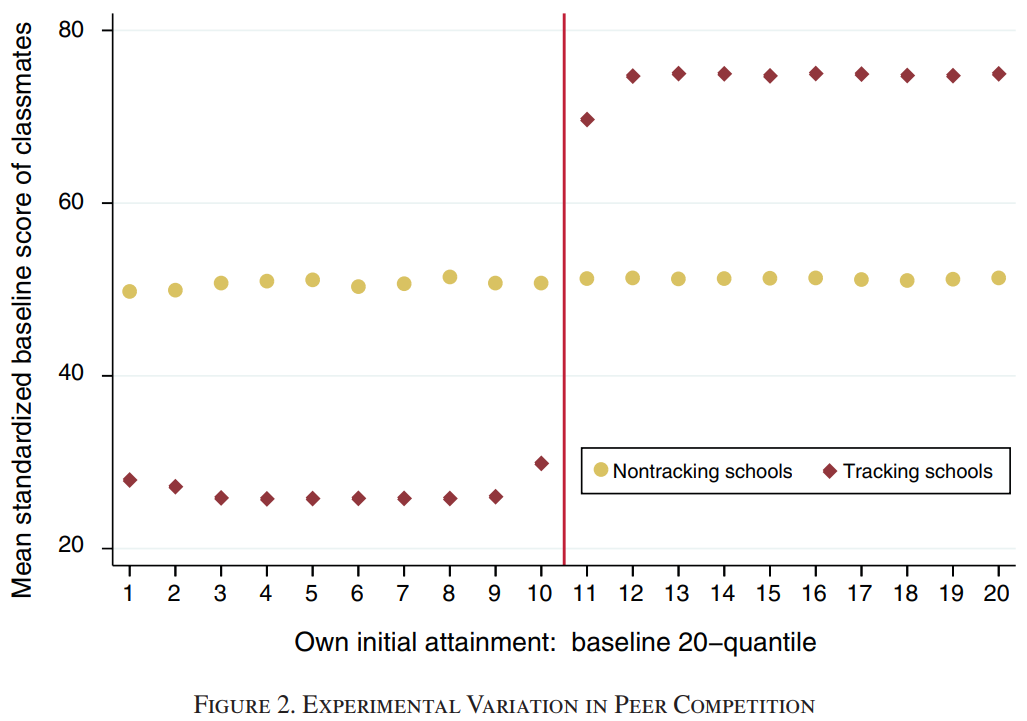
\includegraphics[width= \textwidth]{variation}
\end{frame}


\section{Theoretical model}

\begin{frame}{Model of educational outcome}
  \begin{itemize}
    \item[$y_{ij}:$] The educational outcome of a pupil $i$ in class $j$, given by
  \end{itemize}
  \begin{align}
    y_{ij}=x_{i}+f(\bar{x}_{-ij}) + g(e_{j})h(x_j^{*} - x_{i}) + u_{ij}
    \label{eq:outcome}
  \end{align}
  Where
  \begin{itemize}
    \item[$x_{i}:$] Prior test score of the pupil.
    \item[$\bar{x}_{-ij}:$] Average score of the other pupils in the class. $f(\bar{x}_{-ij}):$ is direct peer effect.
    \item[$e_{j}:$] Teacher's effort. $g(e_{j})$ is concave.
    \item[$x_j^{*}:$] The target level of teacher's instructions depending on class test scores.\\
      $h(\cdot):$ decreases to 0 when the difference between target and pupil's score is $x_j^{*} - x_{i}>\theta$.
    \item[$u_{ij}:$] i.i.d. stochastic pupil- and class-specific factors (symmetric, single-peak).
  \end{itemize}
\end{frame}

\begin{frame}{Teacher's utility maximization problem}
  The teacher decides on effort $e^{*}$ and target level $x^{*}$ to \textbf{maximize utility}.
  \begin{itemize}
    \item[$P(x^{*},e^{*}):$] Payoff function of the distribution of pupils' endline test scores.
    \item[$c(e^{*}):$] Cost function of effort (convex).
    \item[$\lambda>1:$] Contract teachers receive $\lambda$ times more payoff than civil service teachers.
  \end{itemize}
  The empirical results are \textbf{inconsistent} with three special cases $\rightarrow$ decline:
  \begin{itemize}
    \item[-] No direct peer-effects.
    \item[-] No teacher response to class composition.
    \item[-] Teachers payoffs are linear (or concave) in students' endline test scores.
    \comment{Teachers would target the middle of a class, i.e. the just below median pupil would receive worse teaching from tracking.}
  \end{itemize}
  Empirical results are \textbf{consistent} with a model where:
  \begin{itemize}
    \item[$\rightarrow$] Class composition has both direct and indirect effects.
    \item[$\rightarrow$] Teacher's payoffs are convex in student's test scores $\rightarrow$ target top of class.
  \end{itemize}
\end{frame}

\begin{frame}{Anticipated effects of tracking in general}
  The indirect effects depend on whether teachers are incentivized to target the top-, median- or low-achievers in a class (unaffected by treatment).
  \begin{itemize}
    \item High-achieving pupils should gain from tracking.
    \begin{itemize}
      \item[$\uparrow$] Direct student-to-student spillovers.
      \item[$\uparrow$] Indirect effect: Teacher increases effort and level.
    \end{itemize}
    \item Low-achieving pupils could be affected ambiguously
    \begin{itemize}
      \item[$\downarrow$] Less direct student-to-student spillovers.
      \item[$\uparrow$] Indirect effect: Teacher chooses instruction level closer to pupil's ability.
    \end{itemize}
    \item Mid-achieving pupils \textit{above} the median could be affected ambiguously
    \begin{itemize}
      \item[$\uparrow$] Direct student-to-student spillovers
      \item[$\uparrow \downarrow$] Indirect effect: Teacher might increase effort but also increase instruction level above pupil's ability. Depends on teacher's incentives (initial target).
    \end{itemize}
    \item Mid-achieving pupils \textit{below} the median could be affected ambiguously
    \begin{itemize}
      \item[$\downarrow$] Less direct student-to-student spillovers.
      \item[$\uparrow \downarrow$] Indirect effect: Teacher will lower the instruction level. Direction of effect depends on teacher's incentives.
    \end{itemize}
  \end{itemize}
\end{frame}

\begin{frame}{Effects of tracking in Kenya consistent with empirical results}
  Incentive to maximize final scores at the end of \nth{8} grade; many low- and medium-achievers drop out $\Rightarrow$ Kenyan teachers target top-achievers in a class
  \begin{itemize}
    \item High-achieving pupils gain from tracking
    \begin{itemize}
      \item[$\color{green} \uparrow$] Direct student-to-student spillovers.
      \item[$\color{lightgray} \uparrow$] Indirect effect: Teacher increases effort \sout{and level}.
    \end{itemize}
    \item Low-achieving pupils receive a net gain
    \begin{itemize}
      \item[$\color{lightgray} \downarrow$] Less direct student-to-student spillovers.
      \item[$\color{green} \uparrow$] Indirect effect: Teacher chooses instruction level closer to pupil's ability.
    \end{itemize}
    \item Mid-achieving pupils \textit{above} the median receive a net gain
    \begin{itemize}
      \item[$\color{green}\uparrow$] Direct student-to-student spillovers.
      \item[$\color{green}\uparrow \color{lightgray}\downarrow$] Indirect effect: Teacher might increase effort \sout{but also increase instruction level above pupil's ability}. \textit{Teachers initially target top-achievers anyway}.
    \end{itemize}
    \item Mid-achieving pupils \textit{below} the median receive a net gain
    \begin{itemize}
      \item[$\color{lightgray} \downarrow$] Less direct student-to-student spillovers.
      \item[$\color{green}\uparrow \color{lightgray} \downarrow$] Indirect effect: Teacher will lower the instruction level. \textit{Positive effect as teacher now targets mid-achievers as they are the top of the new class.}
    \end{itemize}
  \end{itemize}
\end{frame}

\begin{frame}{Estimation strategy}
  \subsection{Estimation strategy}
  Simple impact of tracking in school $j$ on student $i$'s' test score:
  \begin{align}
    \underbrace{y_{ij}}_\text{Endline test result} = \underbrace{\alpha T_j}_\text{tracking dummy} + \underbrace{X_{ij}\beta}_\text{controls} + \varepsilon_{ij}
  \end{align}
  Control variables $X_{ij}:$ baseline score, gender, age, and contract teacher.

  With interaction between being in a tracking school and in the bottom half $B_{ij}:$
  \begin{align}
    y_{ij} = \alpha T_j + \underbrace{\gamma T_j\times B_{ij}}_\text{interaction term} + X_{ij}\beta + \varepsilon_{ij}
  \end{align}
  i.e. the estimated effect of tracking is
  \begin{itemize}
    \item[$\hat{\alpha}:$] for the top half.
    \item[$\hat{\alpha}+\hat{\gamma}:$] for the bottom half.
  \end{itemize}
\end{frame}

\section{Results}


\begin{frame}{Main results}
  \begin{itemize}
    \item All quartiles benefit from tracking in endline test scores.
    \begin{itemize}
      \item No quartile benefit significantly more than others.
    \end{itemize}
    \item Persistent effects one year after program ended.
    \comment{The classes were united after end-of-funding in all but 5 schools.}
    \begin{itemize}
      \item Overall the effect is slightly, but not significantly larger than endline test.
      \item Lower and insignificant persistent effects for bottom quartile pupils.
    \end{itemize}
  \end{itemize}
\end{frame}


\begin{frame}
  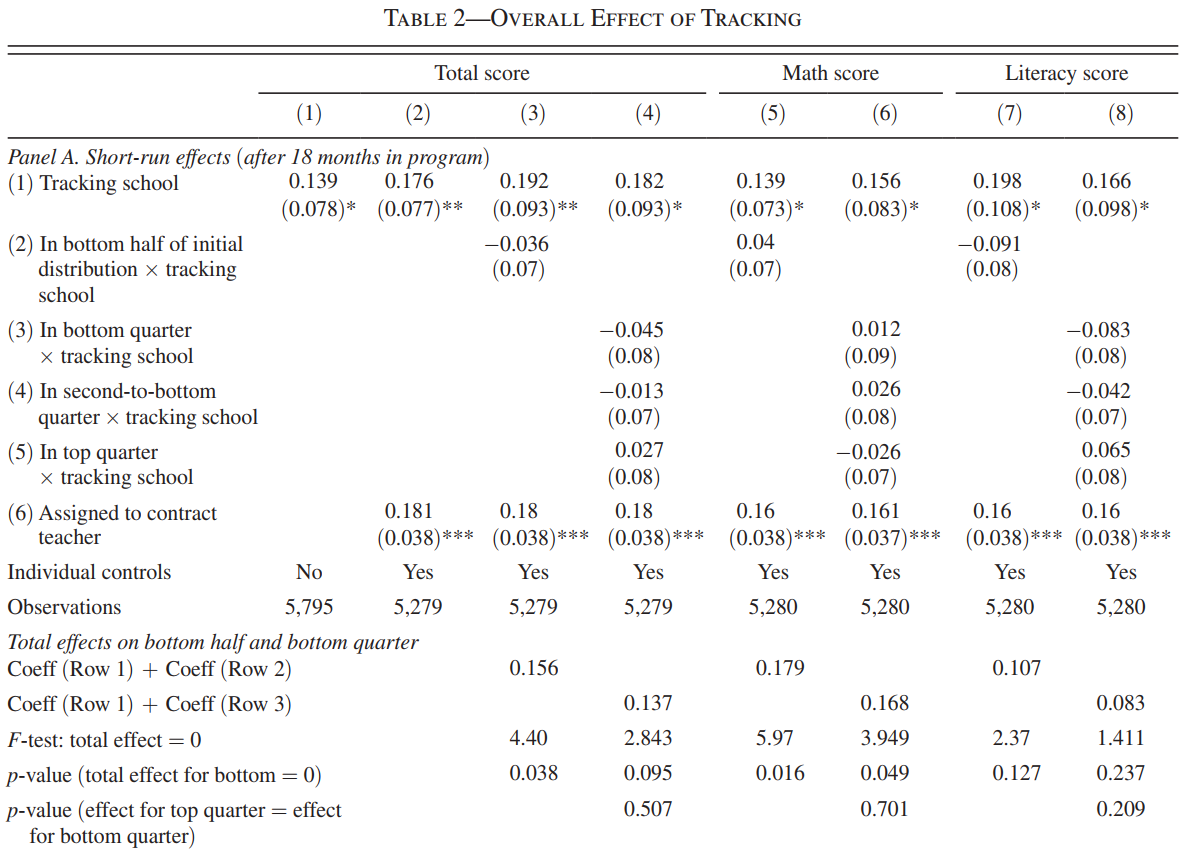
\includegraphics[width= \textwidth]{results}
\end{frame}


\begin{frame}
  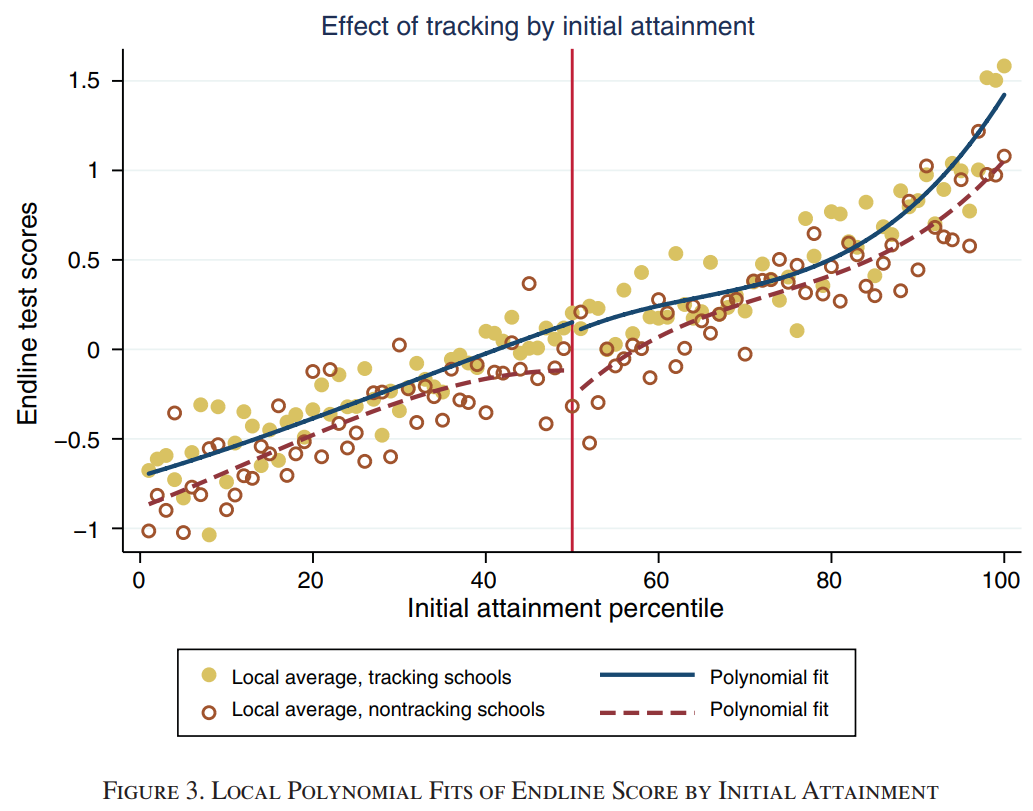
\includegraphics[width= \textwidth]{polynomial}
\end{frame}




\section{Conclusion}


% \begin{frame}{'Endline test' on socrative.com}
%   \subsection{Endline test on socrative.com}
%   ROOM NUMBER:
% \end{frame}


\begin{frame}{Policy implications}
  \subsection{Policy implications}
  \begin{itemize}
    \item Tracking can be beneficial for all pupils if
    \begin{itemize}
      \item Teachers target their instruction to the top of the distribution.
      \item The variation in initial achievement is high.
      \item Direct peer effects are present.
      \item The school initially just had one class per grade.
    \end{itemize}
    \item The combination of an extra teacher and tracking in early years
    \begin{itemize}
      \item Can have persistent effects for top- and mid-achieving pupils.
      \item Low-achieving pupils need continous treatment.
    \end{itemize}
    \item More studies are important to consolidate the robustness of the results.
  \end{itemize}
\end{frame}


\begin{frame}{Econometric takeaways}
  \subsection{Econometric takeaways}
  \begin{itemize}
    \item In a UK study they could not emit selection bias just by controlling for prior test scores \citep{manning2006comprehensive}.
    \begin{itemize}
      \item[$\rightarrow$] Need detailed matching or experimental data with a low level of non-compliers.
    \end{itemize}
    \item 60 different discountinuities provides robustness to the result
    \begin{itemize}
      \item The median pupil will have different achievement levels.
      \item The distribution of peers will be different at different schools.
    \end{itemize}
    % \item For subset (tracking and non-tracking) they look for peer-effects using IV estimation
    % \begin{itemize}
    %   \item
    % \end{itemize}
  \end{itemize}
\end{frame}


\section{References}

\begin{frame}%{References}
  \printbibliography
\end{frame}

%   \begin{figure}[!h]
%   %  \def\svgwidth{0.50\columnwidth}
%   %  \input{tree.pdf_tex}
%     \resizebox{3in}{!}{\input{tree.pdf_tex}}
%   %  \caption{Timeline illustration of event setup}
%   \end{figure}

\end{document}
